\begin{problem}
{\textbf{\textsc{Ambidexterity}}}
When plane-polarized light $\lambda = 500\;\mathrm{nm}$ is passed through a solution with chiral molecules (eg. glucose/DNA), the exiting light is observed to have been rotated by an angle $\Delta \theta$. In chemistry, this optical rotation is measured with a polarimeter device. It is used to measure the relative abundances of left-handed and right-handed molecules, each having their own refractive index $n_L = 1.333333$ and $n_R = 1.333338$ affecting left and right circularly polarized respectively. 

\begin{center}
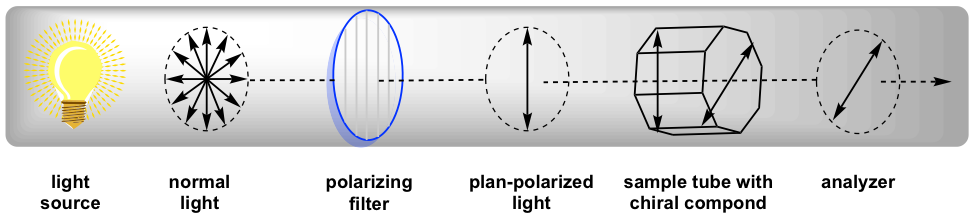
\includegraphics[width=.8\textwidth]{problems/figures/opticalRotationSchematic.png}
\end{center}

If the length of the solution container is $L = 0.15\;\mathrm{m}$, by which angle will the polarization of light rotate, i.e. what is the \textbf{total} optical rotation $\Delta \theta$, in radians? Input the smallest positive answer to this question.
\end{problem}